\noindent{As candidates for events, these possible actions on classes are considered:}
\begin{itemize}
\item Submitting/Cancelling votes:
    When a user votes for a track, or cancels it. If the \textbf{vote} fits within the \textbf{restrictions}, the voted for \textbf{track}s vote count is changed and potentially its order in the \textbf{playlist} class. The specific \textbf{user}s vote is also changed.
\item Checking in/out of venues:
    User checks in at the venue, one wants to vote at. This allows the user to \textbf{vote}.
\item Searching for a track:
    When a user is searching for a desired track in the repertoire/catalogue of tracks. The user should receive relevant search results that fit within the \textbf{restriction}s.
\item Adding/Removing a new track to the playlist:
    If the track a user voted for is not on the playlist already, or if the track only had one vote that got cancelled.
\item New track is playing:
    When a another track instance ended, due to being skipped or reached the end. This should affect the \textbf{vote} count of a \textbf{track}. If a \textbf{user}s track is played his vote should be neglected.
\item Adding/Removing restrictions:
    When the administrator either adds or removes a restriction for the system, this may also be by time intervals. Already added \textbf{track} that does not meet the requirements should be neglected. Cascading through the specific \textbf{users} \textbf{vote}, and the \textbf{playlist}.
\end{itemize}

The following event table is used to describe what classes are involved in the immediate events of the problem domain:

\begin{center}
\label{eventtable}
    \begin{tabular}{|l|l|l|l|l|l|}
    \hline
    \textbf{Events} & User & Track & Playlist & Vote & Restriction \\ \hline
    (Re)vote & * & * & * & * &   \\ \hline
    User checks in at venue & * &   &   & * &   \\ \hline
    User leaves venue & * &   &   &   &   \\ \hline
    User is searching for a track & * &   &   &  & * \\ \hline
    Adding a new track to the playlist & * & * & * & * &   \\ \hline
    Remove track from the playlist & * & * & * & * &   \\ \hline
    A new track is playing & * & * & * & * &   \\ \hline
    Restriction added & * & * & * & * & * \\ \hline
    Restriction removed & * & * & * & * & * \\ \hline
    \end{tabular}
\end{center}

In table \cref{eventtable} the different events in the problem domain and what objects are effected by these are mapped. From this specific state diagrams can be created to illustrate how the objects are created, affected and terminated.

\begin{figure}[H]
  \centering
  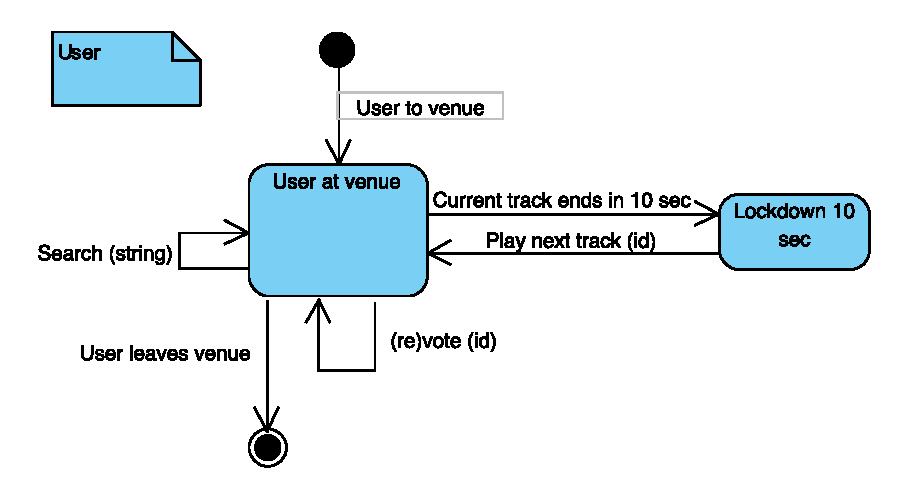
\includegraphics[width=\textwidth]{StateDiagramUser.pdf}
  \caption{State diagram for the user}\label{fig:StateDiagramUser}
\end{figure}
In figure \cref{fig:StateDiagramUser} the state diagram for a user can be seen. The problem domain is the context of the venue, and a user can therefore only affect the problem domain, when he or she is present the venue. This results in the creation of the user, when he or she enters, and the termination when he or she leaves. When present at the venue, the user can search for tracks and vote or revote for these.

\begin{figure}[H]
  \centering
  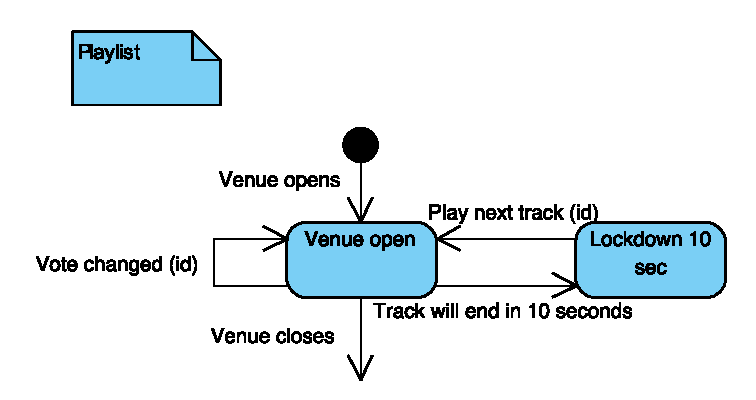
\includegraphics[width=\textwidth]{StateDiagramPlaylist.pdf}
  \caption{State diagram for the playlist}\label{fig:StateDiagramPlaylist}
\end{figure}
In figure \cref{fig:StateDiagramPlaylist} is can be seen that a playlist, is created when the venue opens, and terminated when it closes. To ensure that users can see what the next track will be, without the playlist changing in the last second, and giving the system the time needed to decide the track and change temporary votes to permanent votes, a lockdown is placed 10 seconds before the next track is played, where no user can change their vote. The playlist automatically plays the next track, and when it is not in a lockdown, users can change their votes as desired.

\begin{figure}[H]
  \centering
  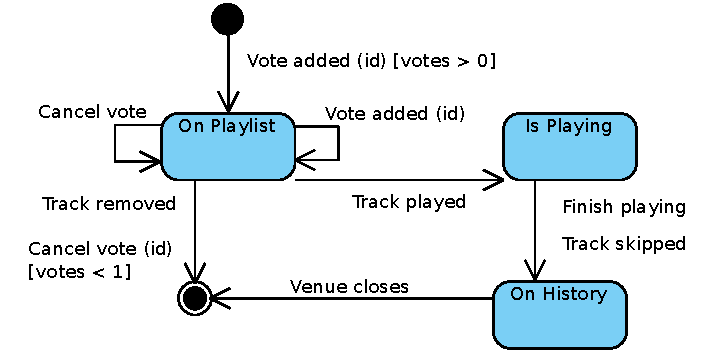
\includegraphics[width=\textwidth]{StateDiagramTrack.pdf}
  \caption{State diagram for the track}\label{fig:StateDiagramTrack}
\end{figure}
As seen in figure \cref{fig:StateDiagramTrack}, a track is only modeled in the problem domain, when it has any votes. This means that it will be created, when it revives its first vote. If temporary votes are removed from the track, it can result in the track having 0 votes again, and will therefore be terminated. While active the track can receive and loose votes from any user, when he or she changes his or her vote. The track will also be terminated when it has been played.

\begin{figure}[H]
  \centering
  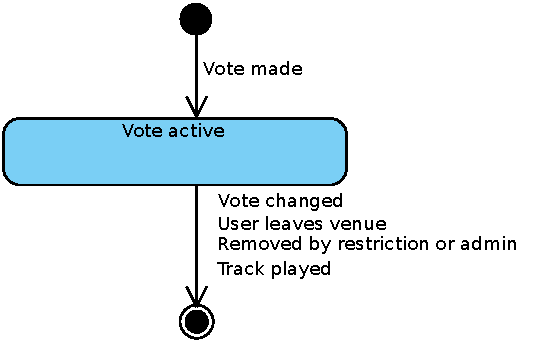
\includegraphics[width=\textwidth]{StateDiagramVote.pdf}
  \caption{State diagram for the vote}\label{fig:StateDiagramVote}
\end{figure}
Figure \cref{fig:StateDiagramVote} illustrates, how votes are affected in the problem domain. A vote is created, when a guest votes on a track for the first time. When the vote is active in its first state, the vote can be changed to which ever track the user can find in a search, resulting in the vote only being temporary for one specific track. When any other track is played, the vote becomes permanent on the one track, and cannot be changed by the user. When this happens, the user will have the ability, to create a new temporary track, by voting on any track. At any time a vote will be terminated, if the user leaves the venue, or the track of which the vote is on is played.

\begin{figure}[H]
  \centering
  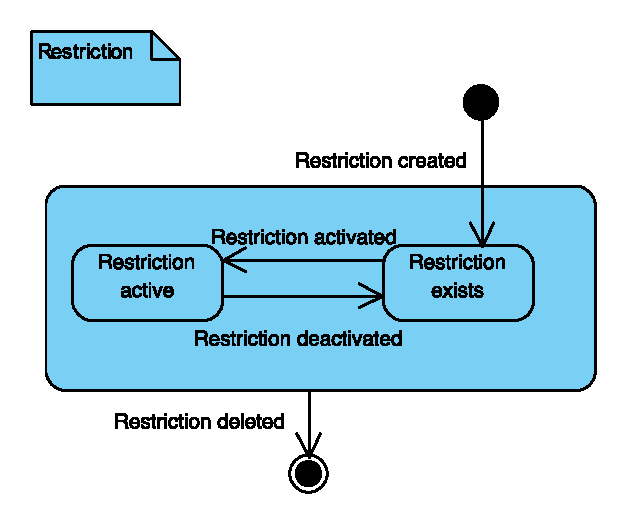
\includegraphics[width=\textwidth]{StateDiagramRestriction.pdf}
  \caption{State diagram for the restriction}\label{fig:StateDiagramRestriction}
\end{figure}
As shown in figure \cref{fig:StateDiagramRestriction}, a restriction can be created and deleted at any time. This can only be done by the administrator. A restriction only affect the users searches when it is active. It can be toggled between active and inactive by the administrator or the system at any time.